\documentclass[12pt]{article}

\usepackage{amsmath}
\usepackage{amsfonts}
\usepackage{float}
\usepackage{fancyhdr}
\usepackage{graphicx}
\usepackage[colorlinks=true,linkcolor=blue, citecolor=red]{hyperref}
\usepackage{url}
\usepackage[top=.75in, left=.5in, right=.5in, bottom=1in]{geometry}
\usepackage[utf8]{vietnam}
\setlength{\headheight}{29.43912pt}

% \graphicspath{PATH_TO_GRAPHIC_FOLDER}

\pagestyle{fancy}
\lhead{
Báo cáo bài tập thực hành 03
}
\rhead{
Trường Đại học Khoa học Tự nhiên - ĐHQG HCM\\
Xử lý ngôn ngữ tự nhiên ứng dụng - CSC15008
}
\lfoot{\LaTeX\ by \href{https://github.com/trhgquan}{Quan, Tran Hoang}}


\begin{document}

% \begin{titlepage}
% \newcommand{\HRule}{\rule{\linewidth}{0.5mm}}
% \centering

% \textsc{\LARGE đại học quốc gia tphcm}\\[1.5cm]
% \textsc{\Large trường đại học khoa học tự nhiên}\\[0.5cm]
% \textsc{\large khoa công nghệ thông tin}\\[0.5cm]
% \textsc{bộ môn công nghệ tri thức}\\[0.5cm]

% \HRule \\[0.4cm]
% { 
% \huge{\bfseries{Báo cáo Bài tập gì gì đấy}}\\[0.5cm]
% \large{\bfseries{Đề tài: Tên đề tài}}
% }\\[0.4cm]
% \HRule \\[0.5cm]

% \textbf{\large Môn học: Tên môn học}\\[0.5cm]

% \begin{minipage}{0.4\textwidth}
% \begin{flushleft} \large
% \emph{Sinh viên thực hiện:}\\
% Trần Sinh Viên (19120338)
% % Nguyễn Văn A \textsc{(19120000)}
% \end{flushleft}
% \end{minipage}
% ~
% \begin{minipage}{0.4\textwidth}
% \begin{flushright} \large
% \emph{Giáo viên hướng dẫn:} \\
% % Dr. James \textsc{Smith}
% Thầy Nguyễn Văn Hướng Dẫn
% \end{flushright}
% \end{minipage}\\[2cm]

% {\large \today}\\[2cm]

% 
\includegraphics{hcmus-logo.png}\\[1cm] 

% \vfill
% \end{titlepage}
	
	
% \tableofcontents
% \pagebreak

\noindent Sinh viên thực hiện: Trần Hoàng Quân - MSSV: 19120338

\section{Giới thiệu ứng dụng Text2Code}
\begin{itemize}
\item \texttt{jupyter-text2code} là một extension của Jupyter Notebook, có chức năng generate ra Python code từ đầu vào là một câu văn bằng ngôn ngữ tự nhiên. 
\item Trang GitHub của ứng dụng: \href{https://github.com/deepklarity/jupyter-text2code}{https://github.com/deepklarity/jupyter-text2code}
\end{itemize}

\subsection{Cài đặt}
Hiện tại ứng dụng chỉ hỗ trợ hệ điều hành MacOS và Ubuntu, tiến hành cài đặt theo hướng dẫn trên trang GitHub của ứng dụng.\footnote{\textbf{Lưu ý:} đối với hệ điều hành Ubuntu, phải cài Miniconda / Anaconda mới có thể cài package \texttt{faiss}}.

\subsection{Chạy thử}
Sau khi cài đặt, thực hiện các bước sau để chạy extension:
\begin{itemize}
\item Khởi chạy jupyter notebook: \texttt{jupyter notebook}
\item Click nút Console: (hình nút console)
\item Nhập câu miêu tả vào input box và nhấn nút \texttt{Text2Code}, code sẽ được generate tự động.
\end{itemize}

\section{Demo}
Trong phần demo, em sẽ sử dụng data từ  \href{https://www.kaggle.com/datasets/imdevskp/corona-virus-report}{bộ dataset COVID-19 trên Kaggle}.
\begin{figure}[H]
    \centering
    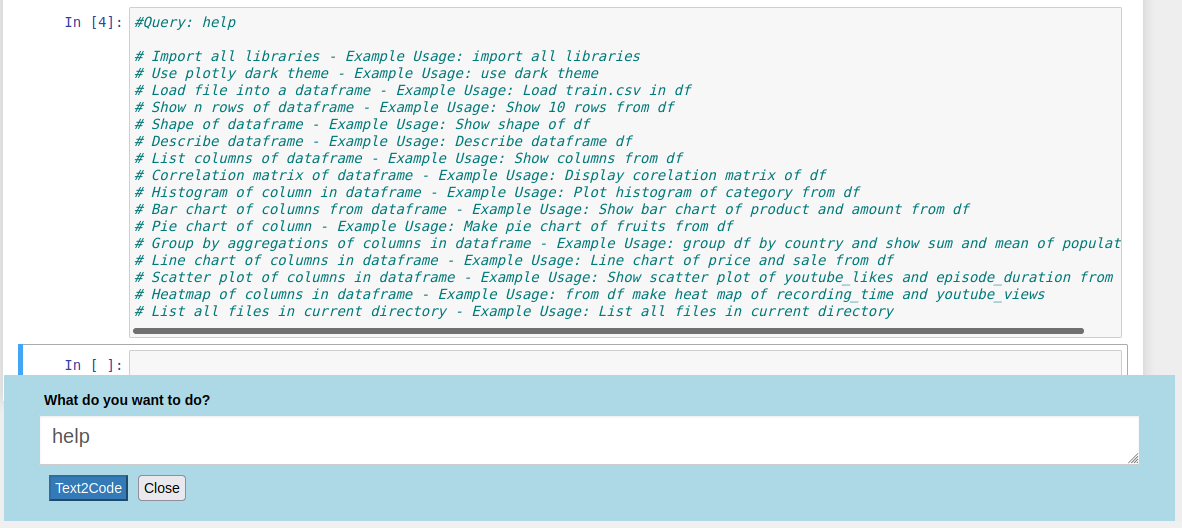
\includegraphics[scale=0.6]{img/help.PNG}
    \caption{Tra cứu danh sách các hàm hỗ trợ: Nhập lệnh \texttt{help}}
\end{figure}
\begin{figure}[H]
    \centering
    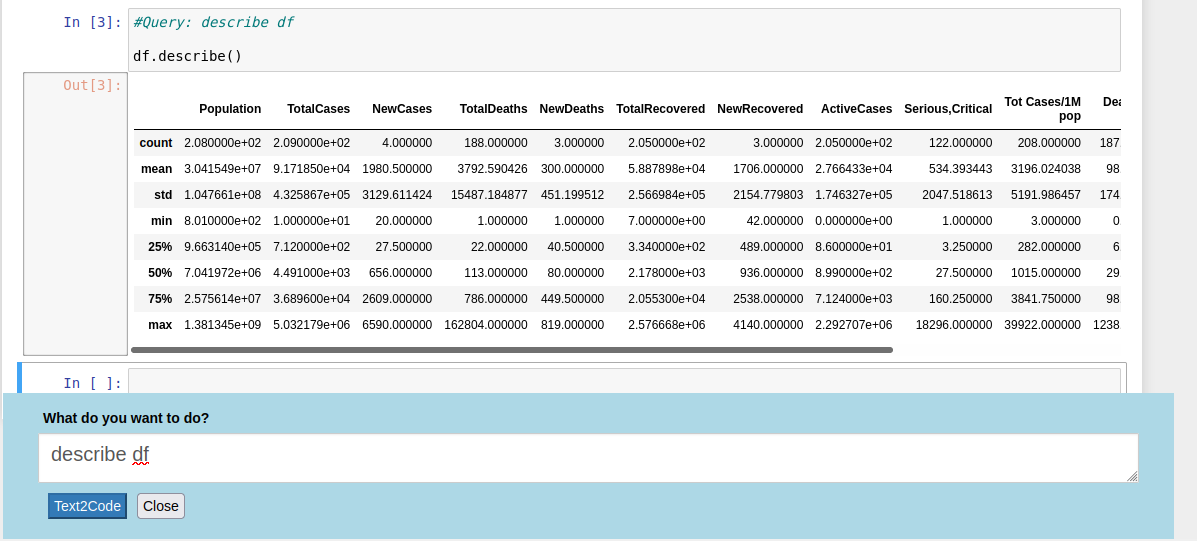
\includegraphics[scale=0.6]{img/describe.PNG}
    \caption{Miêu tả bộ data}
\end{figure}
\begin{figure}[H]
    \centering
    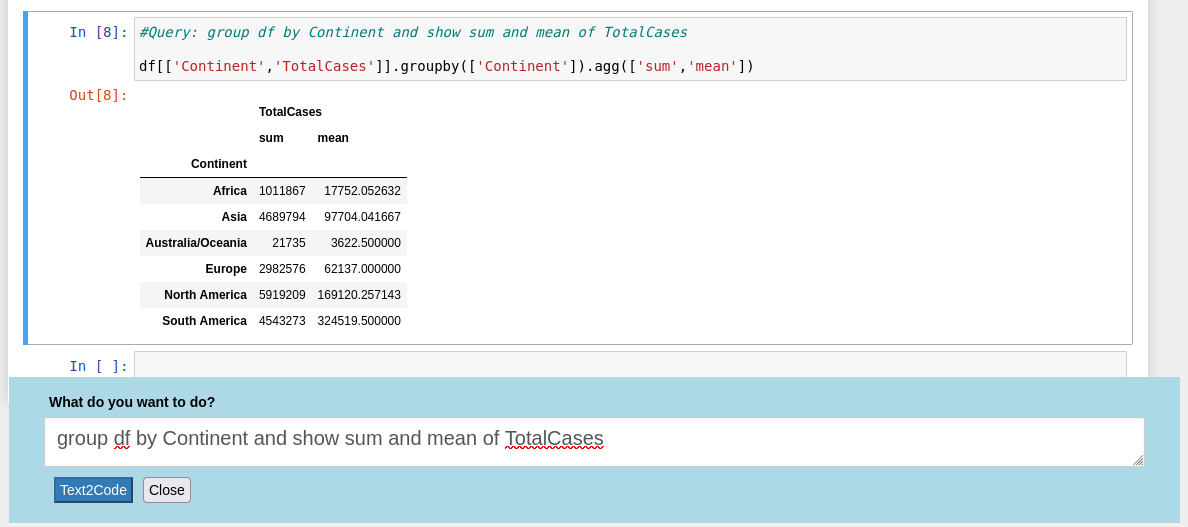
\includegraphics[scale=0.6]{img/complex.PNG}
    \caption{Gom nhóm bởi thuộc tính \texttt{Continent}, sau đó tính tổng số ca mắc và số ca mắc trung bình của từng \texttt{Continent}.}
\end{figure}

\subsection{Video demo}
Vì độ dài nội dung báo cáo có giới hạn, mời Thầy và các bạn xem video demo \href{https://drive.google.com/file/d/1-0ovjPw-pQ_yhcciZBPsEiTubgGCw6MW/view?usp=sharing}{tại link này (Google Drive)} hoặc \href{https://www.youtube.com/watch?v=6i1KpdBGV1I}{tại link này (YouTube)}

\section{Nhận xét}
\begin{itemize}
\item Extension hỗ trợ xử lý và visualise dữ liệu là chính.
\item Nhiều lệnh phải nhập đúng format mới có thể generate đúng ý.
\end{itemize}
\end{document}